\chapter{Kiến trúc và thiết kế hệ thống}
\label{Chapter4}

Chương này trình bày cách nhóm chúng em tổ chức Yoca từ giao diện, máy chủ API đến cơ sở dữ liệu và các nhà cung cấp bên ngoài. Nội dung tập trung vào ranh giới giữa các lớp, hợp đồng dữ liệu, cơ chế lưu đệm và những quyết định giúp hệ thống vận hành ổn định trong giới hạn của các API bên ngoài.

\section{Kiến trúc tổng thể}

Yoca là một ứng dụng web full-stack được quản lý trong cùng một monorepo. Phía người dùng sử dụng React và Vite; phía máy chủ là một ứng dụng Hono chạy trên Node.js, giao tiếp với client qua cả HTTPS lẫn WebSocket; dữ liệu có cấu trúc và cache bền vững được lưu trong PostgreSQL thông qua Drizzle ORM. Backend được triển khai như một monolith, nhưng mã nguồn được chia theo miền như token, pool, wallet, người dùng, cảnh báo, thanh toán và AI. Cách tổ chức này vừa đủ nhẹ cho quy mô nhóm, đồng thời tránh chi phí vận hành nhiều dịch vụ độc lập khi các chức năng vẫn chia sẻ lược đồ và dữ liệu.

\begin{figure}[H]
    \centering
    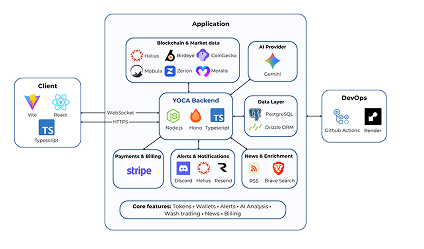
\includegraphics[width=\textwidth]{images/arch.png}
    \caption{Kiến trúc tổng thể và các phụ thuộc bên ngoài của hệ thống Yoca}
    \label{fig:system-architecture}
\end{figure}

Backend đóng vai trò trung chuyển duy nhất; giao diện chỉ trao đổi với API của Yoca. Các phụ thuộc bên ngoài gồm dữ liệu blockchain/thị trường (CoinGecko, Birdeye, Mobula, Zerion, Helius và Moralis), AI (Gemini), PostgreSQL, thanh toán (Stripe), cảnh báo/thông báo (Helius webhook, Resend và Discord) cùng tin tức/enrichment (RSS và Brave News). Khối DevOps nằm ngoài ranh giới \emph{Application} và thể hiện quan hệ build/deploy qua GitHub Actions và Render.

Ranh giới trung chuyển này đặc biệt quan trọng vì mỗi provider có cách biểu diễn token, thời gian, giá trị rỗng và phạm vi lịch sử riêng. Việc chuẩn hóa tại backend giữ những khác biệt đó khỏi các thành phần giao diện.

Các lớp được phân tách theo trách nhiệm nhưng vẫn nằm trong cùng một tiến trình backend. Route tiếp nhận và kiểm tra yêu cầu; service điều phối nghiệp vụ, provider và cache; lớp schema cùng repository quản lý dữ liệu bền vững. Cấu trúc theo miền giúp token, wallet, alert, payment và AI có thể phát triển độc lập về nghiệp vụ mà vẫn dùng chung hợp đồng và hạ tầng vận hành.

\section{Hợp đồng dữ liệu từ giao diện đến nhà cung cấp}

Ứng dụng dùng TypeScript ở cả client và server. Backend xuất kiểu của cây route Hono để client khởi tạo RPC client từ cùng một định nghĩa. Đường dẫn, tham số và kiểu phản hồi nhờ đó được kiểm tra xuyên suốt mà không cần sinh thêm mã từ một đặc tả trung gian. Hono phù hợp với quy mô của Yoca vì kết hợp định tuyến nhẹ với hợp đồng end-to-end trong cùng hệ sinh thái TypeScript \cite{hono}.

Hợp đồng kiểu ở thời điểm phát triển được bổ sung bằng validation runtime tại các biên hệ thống. Tham số từ người dùng và phản hồi của provider được kiểm tra bằng Zod trước khi đi vào phép tính hoặc cơ sở dữ liệu \cite{zod}. Các định danh như token address, wallet address và transaction signature được ràng buộc chặt; metadata hoặc chỉ số biến động được phép thiếu khi nguồn dữ liệu không bảo đảm giá trị. Cách xử lý fail-fast giúp hệ thống từ chối dữ liệu sai cấu trúc trước khi nó ảnh hưởng đến PnL, biểu đồ hoặc kết quả AI.

Lỗi được chuẩn hóa thành một response envelope gồm thông báo, mã lỗi và HTTP status phù hợp. Chi tiết nội bộ của provider không được chuyển nguyên văn ra giao diện; client chỉ cần ánh xạ các nhóm validation, authentication, entitlement, upstream và internal error sang trạng thái hiển thị tương ứng. Với dữ liệu cá nhân, user ID luôn lấy từ phiên xác thực và trở thành điều kiện của truy vấn. Chẳng hạn, thao tác đọc hoặc cập nhật Alert History đồng thời dùng định danh bản ghi và user ID, nhờ đó một tài khoản không thể truy cập lịch sử của tài khoản khác.

Hợp đồng này được áp dụng thống nhất từ route đến service và lớp lưu trữ: route xác nhận request, service trả dữ liệu nội bộ đã chuẩn hóa, còn database bảo vệ ownership cùng các khóa duy nhất. Thay đổi hình dạng response của provider vì vậy được giới hạn tại biên tích hợp.

\section{Luồng truy xuất, chuẩn hóa và lưu đệm}

Luồng truy xuất dữ liệu trước hết kiểm tra bản ghi đã lưu và thời điểm cập nhật. Dữ liệu còn hiệu lực được trả trực tiếp; dữ liệu thiếu hoặc hết hạn được lấy lại từ provider, kiểm tra cấu trúc, chuẩn hóa và ghi vào cơ sở dữ liệu trước khi phản hồi. Cùng một kiểu dữ liệu nội bộ vì vậy được duy trì ở cả hai nhánh, giúp route và giao diện không phụ thuộc vào hình dạng phản hồi của từng nguồn.

Mỗi provider được phân công theo miền dữ liệu phù hợp với thế mạnh và hạn mức sử dụng. CoinGecko và GeckoTerminal cung cấp dữ liệu thị trường, token và pool; Mobula đảm nhiệm PnL, lịch sử hoạt động và tổng giá trị tài sản của ví; Zerion cung cấp chuỗi số dư theo từng token; Helius bổ sung chi tiết giao dịch on-chain và sự kiện webhook. Birdeye và Moralis phục vụ một số tập dữ liệu chuyên biệt. Token metadata có thể được bổ sung từ nhiều nguồn khi cần, còn các phép phân tích chính sử dụng một nguồn ưu tiên để giữ kết quả nhất quán và dễ truy vết.

Cơ sở dữ liệu vừa lưu dữ liệu nghiệp vụ, vừa là lớp cache bền vững. Thiết kế bảng cân bằng mục tiêu chuẩn hóa với số lần gọi API cần thiết để hoàn thiện một bản ghi. Khi các phần dữ liệu có chu kỳ cập nhật khác nhau, chúng được tách thành bảng riêng để chỉ làm mới phần đã cũ. Thông tin hữu ích đi kèm response có thể bổ sung bảng liên quan sau khi đi qua khóa và ràng buộc nhất quán.

\input{Chapter3/database/database}

\section{Lựa chọn công nghệ và giới hạn của thiết kế}

React được chọn vì mô hình thành phần phù hợp với giao diện có nhiều bảng, biểu đồ và trạng thái tương tác dùng lại; Vite cung cấp máy chủ phát triển và cơ chế cập nhật mô-đun nhanh \cite{react,vite}. ECharts đảm nhiệm phần lớn biểu đồ tài chính \cite{echarts}, trong khi các cấu trúc quan hệ giao dịch cần một thành phần đồ thị tương tác riêng. Ở backend, Drizzle được chọn vì cách khai báo lược đồ gần với SQL và cho phép nhóm kiểm soát trực tiếp truy vấn, điều quan trọng khi cache và dữ liệu lịch sử cần các thao tác upsert hoặc truy vấn theo khoảng \cite{drizzle}.

Các lớp kiểm soát được bố trí theo từng ranh giới của hệ thống. Hono RPC duy trì hợp đồng giữa client và server; Zod kiểm tra dữ liệu ở runtime; các ràng buộc cơ sở dữ liệu bảo vệ trạng thái đã lưu; kiểm thử xác nhận hành vi kết hợp giữa các lớp. Cách tổ chức này giúp lỗi về đường dẫn, kiểu dữ liệu và phản hồi bên ngoài được phát hiện gần nơi phát sinh.

Ở phía giao diện, các trang được cấu thành từ lớp truy xuất dữ liệu, trạng thái tương tác và các thành phần trình bày dùng chung. Bảng, biểu đồ và đồ thị giao dịch nhận dữ liệu đã chuẩn hóa từ lớp nghiệp vụ, nhờ đó cùng một chỉ số có thể được sử dụng nhất quán ở Market, Token, Pool và Wallet. Trạng thái tải, dữ liệu rỗng và lỗi được biểu diễn theo cùng quy ước để người dùng luôn nhận biết được kết quả của thao tác.

Localization được tổ chức thành một lớp dùng chung cho nội dung và định dạng. Tiếng Anh và tiếng Việt sử dụng cùng hệ thống khóa; các formatter xử lý thống nhất số, phần trăm, đơn vị token, ngày giờ và tiền tệ. Dữ liệu tài chính được giữ ở đơn vị chuẩn trong API, sau đó lớp hiển thị mới áp dụng locale và quy đổi USD--VND. Thiết kế này hỗ trợ người dùng Việt Nam mà không làm thay đổi các phép tính nghiệp vụ.

\section{Ranh giới tin cậy và các điểm cần bảo vệ}

Yoca tiếp nhận dữ liệu và yêu cầu từ nhiều phía không đáng tin cậy như nhau: người dùng, ví Solana, webhook của provider và mô hình AI. Đăng nhập bằng ví yêu cầu người dùng ký một thông điệp chứa nonce dùng một lần; server xác minh chữ ký ed25519 khớp với public key trước khi cấp phiên đăng nhập, sau đó xóa nonce để tránh dùng lại. Với thanh toán, webhook Stripe được xác thực bằng chữ ký số của Stripe trước khi xử lý sự kiện, còn giao dịch thanh toán bằng Solana được backend truy vấn và đối chiếu địa chỉ nhận, số lượng cùng trạng thái xác nhận trước khi cấp quyền dịch vụ.

Webhook nhận sự kiện ví từ Helius được bảo vệ bằng thông tin xác thực trong header \texttt{Authorization}. Máy chủ kiểm tra thông tin này trước khi xử lý payload, đồng thời sử dụng khóa sự kiện để ngăn một lần gửi lại tạo ra cảnh báo hoặc bản ghi lịch sử trùng lặp.

Đối với AI, ngữ cảnh được xây dựng theo từng miền phân tích và tách khỏi lịch sử hội thoại cùng dữ liệu do công cụ trả về. Nội dung bên ngoài được đặt trong ranh giới rõ ràng để mô hình chỉ tuân theo hướng dẫn hệ thống; phản hồi sau đó được kiểm tra và chuẩn hóa cấu trúc trước khi trả về client. Dữ liệu cá nhân như watchlist, nhãn ví, cảnh báo và lịch sử thanh toán được giới hạn theo user ID đã xác thực như đã trình bày ở phần cơ sở dữ liệu.

\section{Kết chương}

Chương 4 đã xác định Yoca là một monolith phân lớp theo miền, có hợp đồng kiểu xuyên suốt giữa client và server, biên kiểm tra runtime cho dữ liệu bên ngoài và cơ chế lưu trữ ưu tiên tái sử dụng dữ liệu đã đồng bộ. Kiến trúc cân bằng giữa lược đồ chuẩn hóa, hạn mức API, tính nhất quán của dữ liệu và khả năng mở rộng theo miền nghiệp vụ. Trên nền thiết kế đó, Chương 5 trình bày cách hệ thống được triển khai, các chức năng chính và kết quả kiểm thử.
